Die Mischfunktionen in Traverso \Version\ umfassen zur Zeit Volumen, Panorama, Ein- und Ausblenden mit verschiedenen Kurven, trimmen, aufteilen und verschieben von Audioclips, sowie LV2-Plugins für jede Spur. Au"serdem können Audioclips extern mit Sox bearbeitet werden.

\section{Verschieben, trimmen, aufteilen}
Audioclips können mit der Maus durch drücken von \hact{D} frei verschoben werden. Ist das Raster aktiv (\sact{S N}), rasten die beiden Enden jewels am Anfang der Spur, an den Enden anderer Clips, an Markierungen, und am Arbeitscursor ein.

Platziert den Mauszeiger über einem Audioclip und drückt \hact{E}. Dann bewegt die Maus horizontal um das Ende, das sich näher beim Mauszeiger befindet, zu verschieben. Ist das Raster aktiv, rasten auch die Enden auf die oben erwähnten Positionen ein.

Durch \sact{X} werden Audioclips an der Stelle in zwei Clips aufgeteilt, an der sich der Mauszeiger befindet. Die Schnittstelle kann nachträglich mit \hact{E} exakt angepasst werden.

\section{Ein- und Ausblenden}
Beide Enden eines Clips können sanft ein- bzw. ausgeblendet werden. Platziert dazu den Mauszeiger auf dem Clip in der Nähe des Endes, das bearbeitet werden soll, und drückt \hact{F}. Auf der linken Seite wird durch bewegen der Maus eine Einblendkurve erstellt, auf der rechten Seite analog dazu eine Ausblendkurve. Die verschiedenen Formen können mit \sact{M} aufgerufen werden (\FigB~\ref{fig_fades01}).


\begin{figure}[t]
 \centering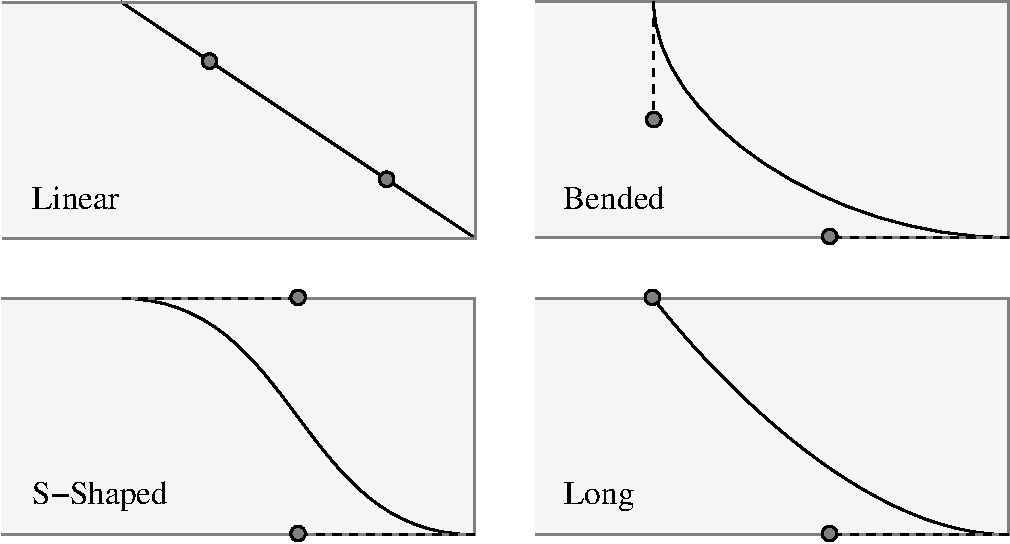
\includegraphics[width=0.8\textwidth]{images/fades}
 \caption{Verschiedene Ein- und Ausblendekurven stehen zur Verfügung. Alle Kurven basieren auf Splines mit zwei Kontrollpunkten (Kreise), deren Position man über die Werte ,,bending'' und ,,strength'' verändern kann.}
 \label{fig_fades01}
\end{figure}

Die verschiedenen Kurven basieren alle auf kubischen Splines mit vier Knotenpunkten. Zwei der Knoten definieren die Stärke der Biegung. Die Position dieser Knoten kann über die zwei Parameter ,,Biegung'' (,,bending'') und ,,Stärke'' (,,strength'') verändert werden. ,,Biegung'' ändert die Richtung der Tangenten in den Endpunkten, wogegen ,,Stärke'' die Gewichtung der Tangenten vorgibt (\FigB~\ref{fig_fades02}). Die Punkte können nicht frei und unabhängig verschoben werden, stattdessen bietet Traverso verschiedene vordefinierte Modi an (\FigB~\ref{fig_fades01}):

\begin{figure}[t]
 \centering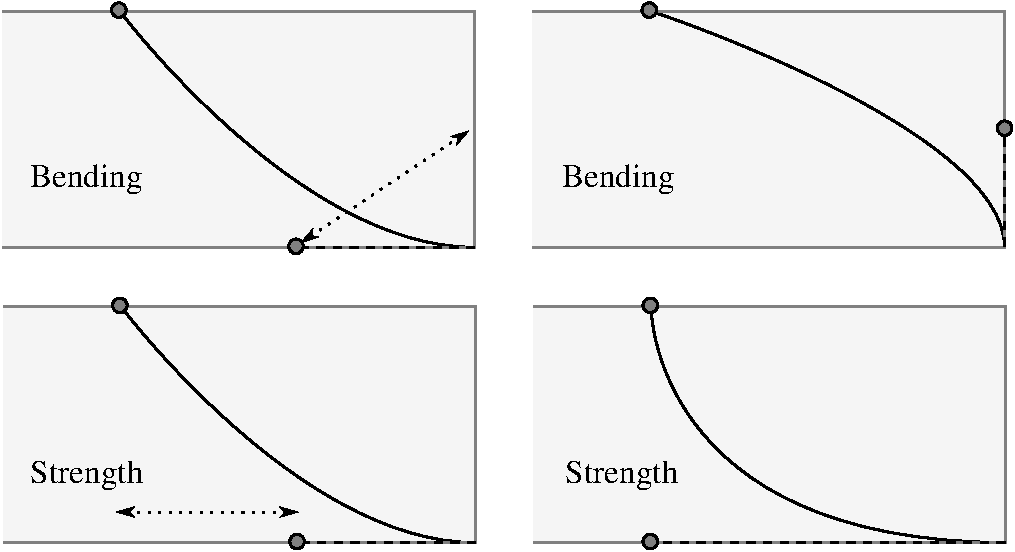
\includegraphics[width=0.8\textwidth]{images/fades2}
 \caption{,,Bending''- und ,,Strength''-Werte dienen dazu, die Form der Ein- und Ausblendekurve zu bearbeiten (hier am Beispiel ,,Long'' gezeigt).}
 \label{fig_fades02}
\end{figure}

\subsection{Linear}
Im linearen Modus bilden die Blendekurven eine gerade Linie zwischen Anfang und Ende des Blendebereichs. Die Kontrollknoten können nicht verschoben werden. Diese Kurven klingen relativ abrupt, besonders am leisen Ende des Bereichs, und werden deshalb eher selten für lange Ausblend-Bereiche am Ende eines Liedes verwendet.

\subsection{S-Form}
S-Kurven starten mit einer horizontalen Tangente, werden im Mittenbereich sehr steil, und gehen am Ende wieder in eine horizontale Tangente über. Anfang und Ende sind sehr weich, aber die schnelle Volumenänderung in der Mitte kann manchmal deutlich hörbar aufallen. Dies kann über die Werte ,,Biegung'' und ,,Stärke'' etwas entschärft werden. Senkrechte Tangenten sind zwar grundsätzlich möglich, ergeben aber in den seltensten Fällen Sinn.

\subsection{Gebogen}
Im gebogenen Modus verläuft jeweils eine Tangente senkrecht und eine waagrecht. Dadurch sind Blenden möglich, die im leisen Bereich sehr flach verlaufen, und im lauten Bereich sehr steil. Über die Werte ,,Biegung'' und ,,Stärke'' kann der Grad der Biegung beeinflusst werden. Sanft ausklingende Ausblendungen sind mit diesem Modus möglich.

\subsection{Lang}
Im ,,Lang''-Modus kann nur der Kontrollpunkt am leisen Ende der Kurve bearbeitet werden. Dieser Modus wird oft für sehr sanfte und lange Ausblendungen verwendet, da er in der Regel durch den sanften Ausklang musikalischer klingt als vergleichbare gebogene oder S-Kurven.

Blenden können zudem numerisch bearbeitet werden. Öffnet dazu den Bearbeitungsdialog des Clips durch drücken von \sact{E}, und wechselt auf die Seite ,,Fades''.

\subsection{Volumenkurve}
Volumenkurven sind ein mächtiges Werkzeug, um den Volumenverlauf eines Audioclips zu bearbeiten. Die Kurven sind fest an die Audioclips gebunden und werden mit diesen mit verschoben. Um eine Volumenkurve zu erstellen oder zu bearbeiten, müssen über den Knopf ,,Effekte anzeigen'' in der oberen Menüleiste die Effekte und Kurven eingeblendet werden (\FigB~\ref{fig_gcurve01}). Standardmä"sig verläuft die Kurve bei 0~dB, am Anfang jedes Clips wird automatisch ein Knoten eingefügt. Weitere Knoten können an der Position des Mauszeigers mit \dact{C} erstellt werden. Die Knoten können auch verschoben \hact{D} und gelöscht \dact{R} werden. Diese Aktionen wirken jeweils auf den Knoten, der sich am nächsten zum Mauszeiger befindet.

\begin{figure}[t]
 \centering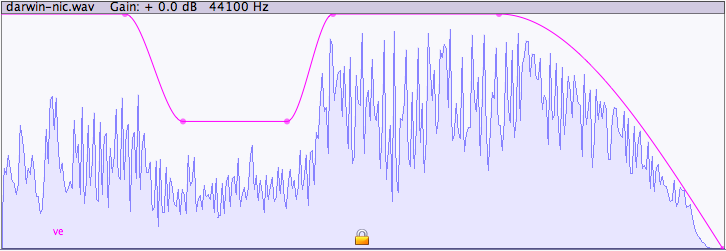
\includegraphics[width=\textwidth]{images/gcurve01}
 \caption{Durch drücken des Knopfes ,,Effekte anzeigen'' in der Menüleisten werden die Volumenkurven angezeigt. Knoten können hinzugefügt, frei verschoben, und gelöscht werden.}
 \label{fig_gcurve01}
\end{figure}

\section{Plugins}
Traverso unterstützt den Plugin-Standard LV2, der die Nachfolge des bekannten LADSPA-Standards antreten wird. Mit \sact{F5} kann ein Dialog aufgerufen werden, der alle installierten LV2-Plugins auflistet (\FigB~\ref{fig_pluglist}). Aktive Plugins werden in der jeweiligen Spur als Kästchen angezeigt. Jedes dieser Felder hat sein eigenes Kontextmenü. Haltet dazu den Mauszeiger über ein Kästchen und drückt \sact{Q} der \sact{Rechte Maustaste}. Mit \sact{E} ruft ihr ein Menü auf, in dem die Plugin-Parameter geändert werden können. Plugins können auch deaktiviert \sact{B} oder gelöscht \dact{R} werden. In Traverso \Version\ werden alle Plugins Post-Fader eingefügt. Weitere Optionen folgen in zukünftigen Versionen.

\begin{figure}[t]
 \centering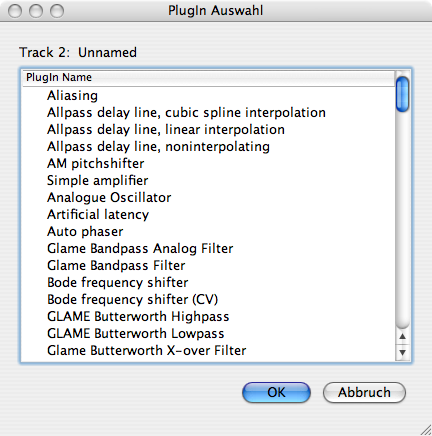
\includegraphics[width=0.6\textwidth]{images/plugin-list}
 \caption{Jeder Spur können Plugins hinzugefügt werden. Der Plugin-Manager wird mit \sact{F5} aufgerufen.}
 \label{fig_pluglist}
\end{figure}


